\documentclass[12pt,letterpaper]{article}

\usepackage[utf8]{inputenc}
\usepackage[T1]{fontenc}
\usepackage[spanish]{babel}
\usepackage[margin=2.54cm]{geometry}
\usepackage{setspace}
\usepackage{titlesec}
\usepackage[hypertexnames=false,bookmarks=false]{hyperref}
\usepackage{helvet}
\usepackage{fancyhdr}
\usepackage{enumitem}
\usepackage{tabularx}
\usepackage{array}
\usepackage{graphicx}
\usepackage{caption}
\captionsetup{font=footnotesize,labelfont=bf,justification=centering}
\graphicspath{{images/}}
\usepackage{placeins}

\setlength{\headheight}{15pt}

\renewcommand{\familydefault}{\sfdefault}

\doublespacing
\setlength{\parindent}{1.27cm}
\setlength{\parskip}{0pt}

\pagestyle{fancy}
\fancyhf{}
\rhead{\thepage}
\renewcommand{\headrulewidth}{0pt}

\titleformat{\section}
{\normalfont\bfseries}
{\thesection.}{0.5em}{}

\titleformat{\subsection}
{\normalfont\bfseries}
{\thesubsection.}{0.5em}{}

\hypersetup{
    colorlinks=true,
    linkcolor=black,
    urlcolor=black
}

\renewcommand{\arraystretch}{1.2}

\begin{document}

\begin{titlepage}
    \centering

    {\large \textbf{UNIVERSIDAD MAYOR DE SAN SIMÓN}}\\
    {\large \textbf{FACULTAD DE CIENCIAS Y TECNOLOGÍA}}\\
    {\large \textbf{CARRERA DE INGENIERÍA INFORMÁTICA}}\\[0.5cm]

    \rule{\textwidth}{0.5pt}\\[0.5cm]
    {\Large \textbf{Trabajo Final -- Semana 2}}\\[0.3cm]
    {\large \textbf{Investigación de usuarios}}\\[0.5cm]
    \rule{\textwidth}{0.5pt}\\[1cm]

    {\large \textbf{Tema}}\\[0.3cm]
    {\large Diseño de una interfaz administrativa para el control de distribución presencial de guías académicas en la Carrera de Física}\\[2cm]

    \begin{flushleft}
        \textbf{Integrantes:}\\
        \hspace*{0.5cm}\textbullet\ José Daniel Virreira Rufino\\
        \hspace*{0.5cm}\textbullet\ Mairon Henry Fernandez Orellana\\
        \hspace*{0.5cm}\textbullet\ Jonas Vidal Zenzano\\
        \hspace*{0.5cm}\textbullet\ Luis Fernando Cardenas Morales
    \end{flushleft}

    \begin{flushleft}
        \textbf{Grupo:} UXploradores\\
        \textbf{Materia:} Interacción Humano-Computadora\\
        \textbf{Docente:} Mgr. Corina Flores Villarroel\\
        \textbf{Gestión:} I-2026
    \end{flushleft}

    \vfill

    {\small Cochabamba -- Bolivia}\\
\end{titlepage}

El presente informe corresponde a la etapa de investigación de usuarios del proyecto. El objetivo de esta fase fue conocer mejor a las personas relacionadas con el proceso de distribución presencial de guías académicas de Física, identificando sus necesidades, dificultades y expectativas frente al sistema actual de control. Para ello, se consideraron dos grupos de usuarios: los encargados del Centro de Estudiantes de Física, como usuarios principales del sistema administrativo, y los estudiantes compradores, como usuarios secundarios dentro del proceso de compra presencial.

\section{Metodología}

La investigación se realizó mediante encuestas aplicadas a los dos grupos de usuarios identificados. En primer lugar, se aplicó una encuesta a estudiantes compradores de guías de laboratorio de Física, con un total de 25 respuestas. Esta encuesta permitió conocer la experiencia de compra presencial, la claridad sobre la disponibilidad de guías y las principales dudas que tienen los estudiantes antes de acercarse al Centro de Estudiantes.

En segundo lugar, se aplicó una encuesta a encargados del Centro de Estudiantes de Física, con un total de 7 respuestas. Esta encuesta se enfocó en el uso del sistema actual de control de guías, entendido como una planilla de Excel con funciones automatizadas. La intención no fue desvalorizar dicho sistema, sino identificar qué aspectos resultan útiles, qué elementos conviene conservar y qué necesidades podrían considerarse en una futura propuesta de interfaz administrativa.

A continuación, presentamos los resultados más relevantes de ambas encuestas, organizados en torno a las necesidades y problemas detectados para cada grupo de usuarios. Además, se incluyen escenarios de uso que reflejan situaciones comunes dentro del proceso de distribución presencial de guías académicas:

% --- Inserción de figuras seleccionadas (encargados y compradores) ---
% Mostrar cada imagen como figura individual, con caption descriptivo y breve descripción
\begin{figure}[!htbp]
    \centering
    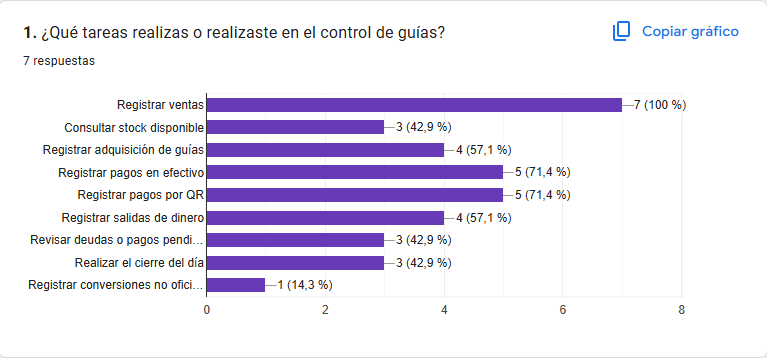
\includegraphics[width=0.8\textwidth]{pregunta_1_encargados.png}
    \caption{Encargados — Pregunta 1: Distribución de tareas realizadas (ventas, inventario, cierres).}
    \label{fig:preg1_enc}
\end{figure}

\begin{figure}[!htbp]
    \centering
    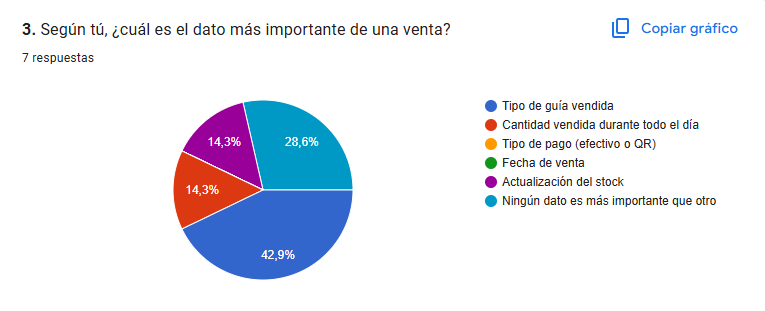
\includegraphics[width=0.8\textwidth]{pregunta_3_encargados.png}
    \caption{Encargados — Pregunta 3: Frecuencia de tareas complementarias (pagos, salidas, adquisiciones).}
    \label{fig:preg3_enc}
\end{figure}

\begin{figure}[!htbp]
    \centering
    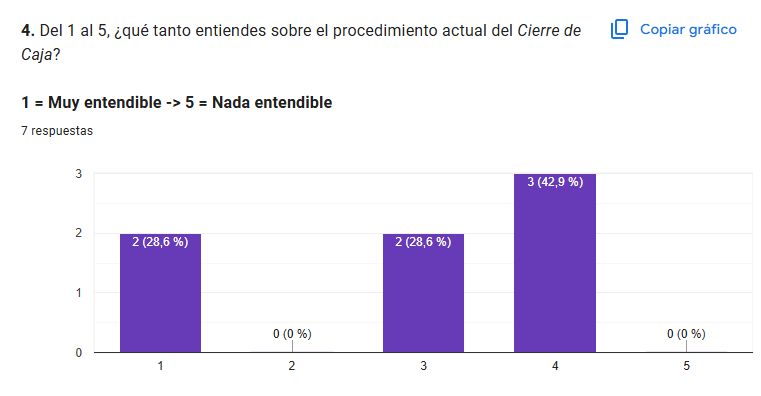
\includegraphics[width=0.8\textwidth]{pregunta_4_encargados.png}
    \caption{Encargados — Pregunta 4: Claridad del cierre de caja (escala de entendimiento).}
    \label{fig:preg4_enc}
\end{figure}

\begin{figure}[!htbp]
    \centering
    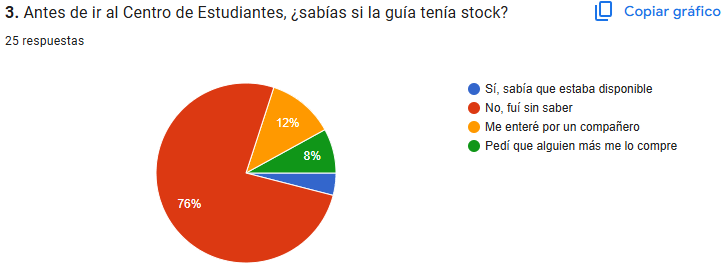
\includegraphics[width=0.8\textwidth]{pregunta_3_compradores.png}
    \caption{Compradores — Pregunta 3: Proporción de estudiantes por materia (Física General, Física Básica I/II/III).}
    \label{fig:preg3_comp}
\end{figure}

\begin{figure}[!htbp]
    \centering
    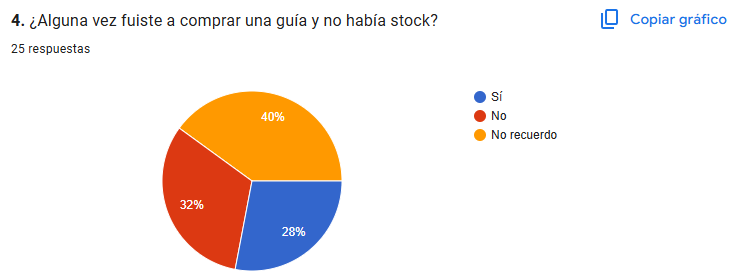
\includegraphics[width=0.8\textwidth]{pregunta_4_compradores.png}
    \caption{Compradores — Pregunta 4: Dudas sobre disponibilidad antes de acudir (sí/no).}
    \label{fig:preg4_comp}
\end{figure}

\begin{figure}[!htbp]
    \centering
    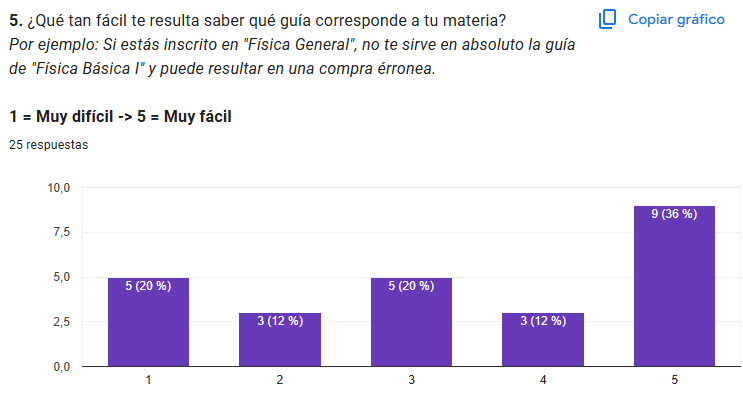
\includegraphics[width=0.8\textwidth]{pregunta_5_compradores.png}
    \caption{Compradores — Pregunta 5: Otras dificultades reportadas (identificación de guía, información previa).}
    \label{fig:preg5_comp}
\end{figure}

\newpage

\subsection{Instrumento (preguntas clave)}
Breve resumen de preguntas incluidas en la encuesta (reemplaza por redacción exacta si lo prefieres):
\begin{itemize}
    \item ¿Confirmó disponibilidad de la guía antes de acudir al Centro? (sí/no)
    \item ¿Con qué claridad entiende el procedimiento de cierre de caja? (escala 1–5)
    \item ¿Tuvo dificultad para identificar qué guía correspondía a su materia? (sí/no)
    \item ¿Con qué frecuencia se registran ventas manualmente en el sistema actual? (opciones)
    \item ¿Qué información le gustaría ver antes de acudir a comprar? (pregunta abierta, categorías)
\end{itemize}
\vspace{-0.5em}

\section{Perfil de usuarios}

Los usuarios principales del sistema son los encargados del Centro de Estudiantes de Física. Ellos realizan tareas administrativas relacionadas con la distribución de guías, como registrar ventas, consultar stock, registrar pagos en efectivo o QR, controlar salidas de dinero, revisar deudas y realizar el cierre del día. Según la encuesta, el 100\% de los encargados participa en el registro de ventas, mientras que otras tareas como registrar adquisiciones, pagos o salidas de dinero aparecen en más de la mitad de las respuestas.

\begin{center}
\begin{tabularx}{\textwidth}{|>{\bfseries}p{4cm}|X|}
\hline
Arquetipo & Encargado del Centro de Estudiantes de Física \\
\hline
Rol & Usuario principal del sistema administrativo. \\
\hline
Objetivo & Registrar y controlar correctamente las ventas, el stock, los pagos y el cierre de caja. \\
\hline
Necesidades & Contar con información clara, organizada y confiable sobre ventas, inventario, dinero disponible y movimientos realizados. \\
\hline
Dificultades & Comprender algunos procedimientos administrativos, especialmente el cierre de caja, y verificar registros anteriores cuando existe duda. \\
\hline
\end{tabularx}
\end{center}

El segundo grupo corresponde a los estudiantes compradores. Ellos no usarán directamente el sistema administrativo, pero forman parte del proceso de distribución presencial de guías. Su participación permite comprender mejor el contexto de compra y las dudas más frecuentes antes de ir al Centro de Estudiantes.

\begin{center}
\begin{tabularx}{\textwidth}{|>{\bfseries}p{4cm}|X|}
\hline
Arquetipo & Estudiante comprador de guías de Física \\
\hline
Rol & Usuario secundario dentro del proceso de compra presencial. \\
\hline
Objetivo & Comprar la guía correcta de laboratorio de acuerdo con la materia que cursa. \\
\hline
Necesidades & Saber si existe stock disponible, identificar qué guía corresponde a su materia y conocer información básica antes de acercarse al Centro. \\
\hline
Dificultades & Incertidumbre sobre disponibilidad de guías y confusión sobre qué guía corresponde a cada materia. \\
\hline
\end{tabularx}
\end{center}

En la encuesta a compradores participaron estudiantes de distintas carreras. Las respuestas más frecuentes provinieron de Ingeniería Informática, Licenciatura en Física e Ingeniería de Sistemas. Respecto a las materias, predominan Física General con 44\% y Física Básica III con 40\%.

\section{Necesidades identificadas}

A partir de las encuestas, se identificaron necesidades distintas para cada grupo de usuario.

En el caso de los encargados del Centro de Estudiantes, las principales necesidades se relacionan con el control administrativo. Los resultados muestran que el sistema debe permitir manejar correctamente ventas, stock, pagos, salidas de dinero y cierre de caja. Además, los encargados valoran que un sistema sea fácil de entender desde el primer uso, que tenga pocas pantallas u opciones, y que muestre la información de forma ordenada.

También se identificó la necesidad de conservar aspectos positivos del sistema actual, como su automatización, la organización de funciones, la visibilidad del stock y el uso de botones para realizar acciones. Una respuesta relevante señala que sería útil contar con un historial para saber si se presionó por accidente algún botón o si se registró una acción no deseada.

En el caso de los estudiantes compradores, la necesidad principal es contar con información previa antes de ir al Centro de Estudiantes. El 76\% indicó que fue sin saber si la guía tenía stock. Además, el 32\% señaló que la parte menos clara del proceso es saber si la guía aún está disponible, mientras que el 24\% indicó dificultad para identificar qué guía corresponde a su materia.

\begin{center}
\begin{tabularx}{\textwidth}{|>{\bfseries}p{5cm}|X|}
\hline
Encargados & Necesitan claridad en el control de ventas, stock, pagos, salidas de dinero, cierre de caja e historial de acciones. \\
\hline
Compradores & Necesitan saber disponibilidad de guías, correspondencia entre guía y materia, y datos básicos antes de ir al Centro. \\
\hline
\end{tabularx}
\end{center}

\section{Problemas detectados}

En los encargados, el problema más importante se relaciona con la comprensión del cierre de caja. En la escala utilizada, donde 1 significaba muy entendible y 5 nada entendible, el 42.9\% marcó el valor 4. Esto indica que el procedimiento no resulta completamente claro para una parte importante de los usuarios principales.

También se detectó que, aunque el sistema actual tiene elementos útiles, algunos procesos requieren mayor seguridad y trazabilidad. La respuesta abierta relacionada con saber si se presionó accidentalmente un botón muestra una posible necesidad de historial o confirmación de acciones.

En los compradores, el problema más evidente es la falta de información previa sobre stock. La mayoría no sabía si la guía estaba disponible antes de ir al Centro de Estudiantes. Además, un 28\% indicó que alguna vez fue a comprar una guía y no había stock. Otro problema detectado es la dificultad para identificar qué guía corresponde a cada materia, especialmente porque no todas las carreras cursan las mismas materias de Física.

\begin{center}
\begin{tabularx}{\textwidth}{|>{\bfseries}p{5cm}|X|}
\hline
Problema administrativo & El cierre de caja no es completamente entendible para todos los encargados. \\
\hline
Problema de control & Se necesita mayor trazabilidad para revisar acciones realizadas dentro del sistema. \\
\hline
Problema de información & Los estudiantes no siempre saben si existe stock disponible antes de ir a comprar. \\
\hline
Problema de orientación & Algunos estudiantes no tienen claro qué guía corresponde a su materia. \\
\hline
\end{tabularx}
\end{center}

\section{Escenarios de uso}

\subsection{Escenario 1: Registro de venta de una guía}

Un estudiante se acerca al Centro de Estudiantes de Física para comprar una guía de laboratorio. El encargado consulta el tipo de guía solicitada, registra la venta en el sistema actual, selecciona el tipo de pago correspondiente y entrega la guía física. El sistema debe actualizar el stock y reflejar el movimiento de dinero de forma clara.

\subsection{Escenario 2: Consulta de disponibilidad}

Antes o durante la atención, el encargado necesita verificar si una guía se encuentra disponible. Para ello revisa el stock actual y confirma si existe cantidad suficiente. Este escenario es importante porque los compradores indicaron que una de sus principales dudas es saber si la guía aún está disponible.

\subsection{Escenario 3: Cierre de caja}

Al finalizar la jornada, el encargado revisa las ventas realizadas, los pagos en efectivo, los pagos por QR, las salidas de dinero y el dinero disponible. Luego realiza el cierre de caja. Este escenario requiere especial claridad, ya que los resultados de la encuesta muestran que el procedimiento no es completamente entendible para todos los encargados.

\subsection{Escenario 4: Identificación de la guía correcta}

Un estudiante necesita comprar una guía, pero no está seguro de cuál corresponde a su materia. El sistema o la información disponible debería ayudar a relacionar cada materia con su guía correspondiente, evitando compras incorrectas o consultas repetidas.

En síntesis, la investigación muestra que el proyecto debe mantenerse enfocado en los encargados del Centro de Estudiantes como usuarios principales. El sistema actual cumple funciones importantes y debe tomarse como base, especialmente por su automatización y organización. Sin embargo, existen oportunidades para hacer más clara la información, mejorar la trazabilidad de acciones, facilitar el cierre de caja y ofrecer datos básicos que reduzcan la incertidumbre de los compradores.

\end{document}